\section{Geschwindigkeitsbasiertes Bewegungsmodell } \footnote{Das Bewegungsmodell und dessen Herleitung stammen aus \cite[S. 121 ff]{ProbRob}} 
Als erstes Beispiel wird ein stochastisches Modell für die Roboterbewegung entworfen, wobei anhand des vergangenen Positionsvektor $\mVec{x}_{t-1}$ und des aktuellen Steuervektors $\mVec{u}_t$ die Wahrscheinlichkeitsverteilung des aktuellen Positionsvektors $\mVec{x}_t$
\begin{equation}
\condP{\mVec{x}_t}{\mVec{u}_t, \mVec{x}_{t-1}}
\end{equation}
bestimmt werden soll. In diesem Fall wird lediglich eine planare Bewegung betrachtet, das heißt der Roboter bewegt sich in der xy-Ebene. Der Positionsvektor setzt sich somit aus den drei Größen
\begin{equation}
\mVec{x} = \begin{pmatrix}
x \\ y \\ \theta
\end{pmatrix}
\end{equation}
zusammen, welche die x-/y-Position und Ausrichtung des Roboters wiedergeben. $\theta$ gibt dabei den Winkel zwischen der x-Koordinatenachse und der Blickrichtung des Roboters an.
Der Steuervektor $\mVec{u}$ gibt die aktuelle Translations- und Rotationsgeschwindigkeit
\begin{equation}
\mVec{u} = \begin{pmatrix}
v \\ \omega
\end{pmatrix}
\end{equation}
des Roboters an, wobei angenommen wird, dass die beiden Geschwindigkeiten zwischen zwei Abtastpunkten $t$ und $t+1$ konstant sind. $v$ beschreibt die Translationsgeschwindigkeit in Blickrichtung, während $\omega$ die Änderung des Blickwinkels $\theta$ wiedergibt.
Unter der Annahme dass die Geschwindigkeiten $\mVec{u}$ in dem Intervall $]t-1, t]$ zwischen zwei Abtastpunkten konstant bleibt, kann die Bewegung als Rotation um einen konstanten Momentanpol $\mVec{c} = \begin{pmatrix} x_c & y_c \end{pmatrix}^T$ betrachtet werden.
\begin{figure}[!ht]
\centering
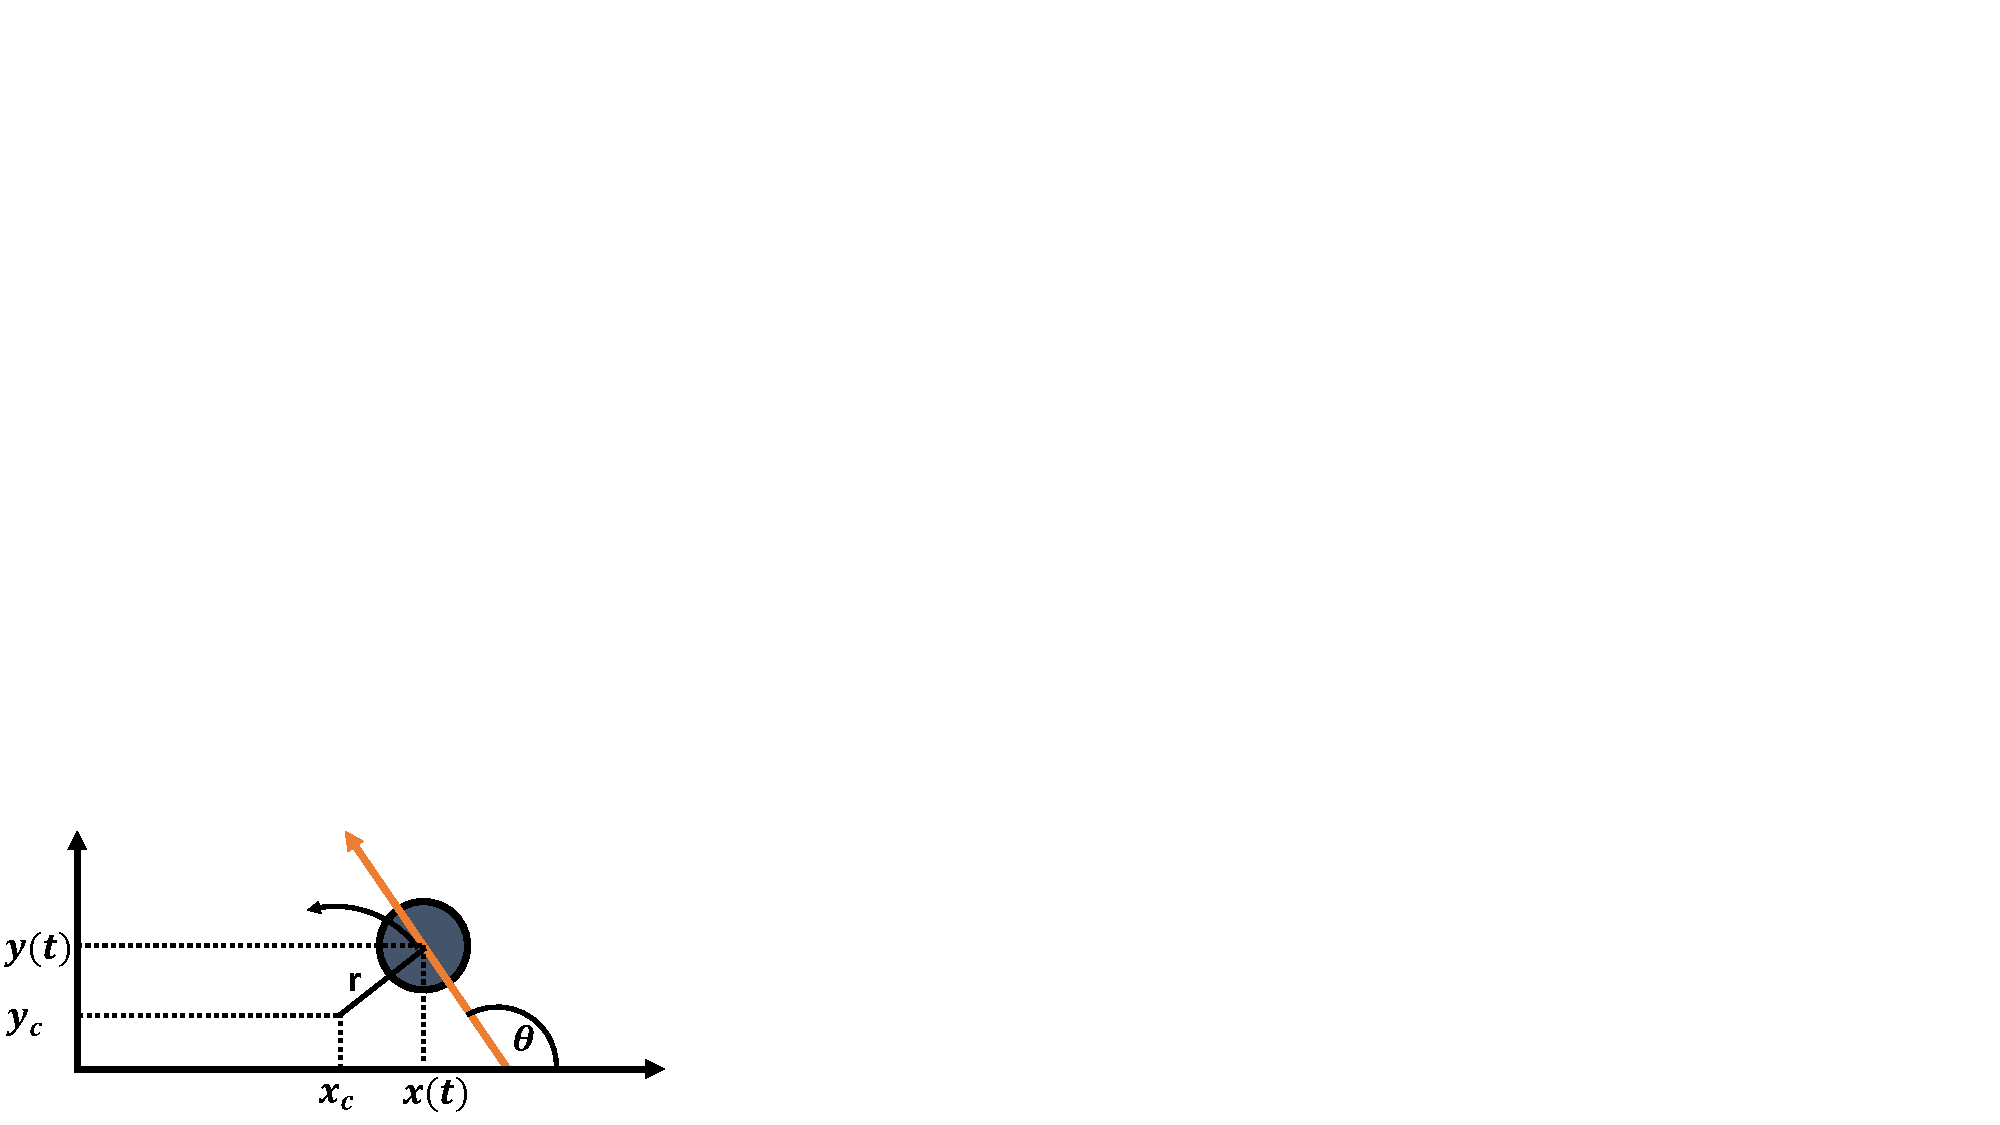
\includegraphics[width=0.6\linewidth, trim={0cm 0cm 24cm 14cm}, clip]{img/Bild_Kinematik_1}
\caption{Darstellung des Momentanpols am Zeitpunkt $t$ \cite[S. 126]{ProbRob}}
\end{figure}

Für den Radius gilt
\begin{equation}
r = \left\vert \frac{v}{\omega}\right\vert\,,
\end{equation}
wobei zu beachten ist, dass der Radius für eine Winkelgeschwindigkeit $\omega=0$ gegen unendlich konvergiert, was wiederum einer reinen Translation entspricht. Aus dem Positionsvektors des Roboters $\mVec{x}_t$ an dem Zeitpunkt $t$ kann der Momentanpol für die folgende Abtastperiode berechnet werden:
\begin{equation}
\label{eq_kinematic_1}
\begin{pmatrix}
x_c \\ y_c
\end{pmatrix} = \begin{pmatrix}
x(t) - \frac{v}{\omega}\cdot \mySin{\theta} \\ y(t) + \frac{v}{\omega}\cdot \myCos{\theta}
\end{pmatrix} \hspace{15pt}\leftrightarrow\hspace{15pt} 
\begin{pmatrix}
x(t) \\ y(t)
\end{pmatrix} = \begin{pmatrix}
x_c + \frac{v}{w}\cdot \mySin{\theta} \\ y_c - \frac{v}{w}\cdot \myCos{\theta}
\end{pmatrix}\,.
\end{equation}
Im nächsten Schritt wird die Bewegung über eine Abtastperiode $\Delta t$ betrachtet, wodurch der Roboter um die Winkeldifferenz $\Delta t\cdot \omega$ auf dem Kreisbogen wandert. Nach \ref{eq_kinematic_1} folgt für den Positionsvektor am Zeitpunkt $t+\Delta t$
\begin{equation}
\label{eq_kinematic_2}
\begin{split}
\begin{pmatrix}
x(t+\Delta t) \\ y(t+\Delta t) \\ \theta(t+\Delta t
\end{pmatrix} &= \begin{pmatrix}
x_c + \frac{v}{w}\cdot \mySin{\theta(t)+\omega\cdot \Delta t} \\ y_c - \frac{v}{w}\cdot \myCos{\theta(t)+\omega \cdot \Delta t} \\ \theta(t) + \omega\cdot \Delta t
\end{pmatrix}\\
& = \begin{pmatrix}
x(t) \\ y(t) \\ \theta(t)
\end{pmatrix} + \begin{pmatrix}
-\frac{v}{\omega}\cdot\mySin{\theta(t)} + \frac{v}{\omega}\cdot \mySin{\theta(t)+\omega \cdot \Delta t} \\
\frac{v}{\omega}\cdot \myCos{\theta(t)} - \frac{v}{w}\cdot \myCos{\theta(t)+\omega \cdot \Delta t}\\
\omega\cdot \Delta t
\end{pmatrix}\,.
\end{split}
\end{equation}
Bisher wurden lediglich deterministische Bewegungen betrachtet. Um nun mögliche Fehler des Steuervektors $\mVec{u}$ zu beachten, werden die störbehafteten Geschwindigkeiten
\begin{equation}
\mVec{u} = \begin{pmatrix}
\hat{v} \\ \hat{\omega}
\end{pmatrix} = \begin{pmatrix}
v + v\idx{err} \\ \omega + \omega\idx{err}
\end{pmatrix}
\end{equation}
eingeführt. Die Zufallsvariablen $v\idx{err}$ und $\omega\idx{err}$ dienen der Fehlermodellierung und ihre Wahrscheinlichkeitsverteilungen $\varepsilon_v$ und $\varepsilon_\omega$ werden dem Anwendungsfall nach angepasst. Einsetzen des stochastischen Steuervektors $\mVec{u}$ liefert
\begin{equation}
\begin{pmatrix}
x(t+\Delta t) \\ y(t+\Delta t) \\ \theta(t+\Delta t
\end{pmatrix} 
=
\begin{pmatrix}
x(t) \\ y(t) \\ \theta(t)
\end{pmatrix} + \begin{pmatrix}
-\frac{\hat{v}}{\hat{\omega}}\cdot\mySin{\theta(t)} + \frac{\hat{v}}{\hat{\omega}}\cdot \mySin{\theta(t)+\hat{\omega} \cdot \Delta t} \\
\frac{\hat{v}}{\hat{\omega}}\cdot \myCos{\theta(t)} - \frac{\hat{v}}{w}\cdot \myCos{\theta(t)+\hat{\omega} \cdot \Delta t}\\
\hat{\omega}\cdot \Delta t
\end{pmatrix}\,.
\end{equation}
In diesem Modell wurden lediglich zwei Zufallsvariablen eingeführt, um die Störung von drei Positionsvariablen zu modellieren. Aus diesem Grund entsteht eine ungewollte stochastische Abhängigkeit zwischen den Elementen des Positionsvektors $\mVec{x}(t+\Delta t)$. Dieses Problem wird behoben, indem eine dritte Zufallsvariable
\begin{equation}
\gamma\idx{err} \equiv \hat{\gamma}
\end{equation}
eingeführt wird, die zu einer zusätzlichen Störung der Orientierung $\theta(t+\Delta t)$ in Form von
\begin{equation}
\label{eq_kinematic_3}
\begin{pmatrix}
x(t+\Delta t) \\ y(t+\Delta t) \\ \theta(t+\Delta t
\end{pmatrix} 
=
\begin{pmatrix}
x(t) \\ y(t) \\ \theta(t)
\end{pmatrix} + \begin{pmatrix}
-\frac{\hat{v}}{\hat{\omega}}\cdot\mySin{\theta(t)} + \frac{\hat{v}}{\hat{\omega}}\cdot \mySin{\theta(t)+\hat{\omega} \cdot \Delta t} \\
\frac{\hat{v}}{\hat{\omega}}\cdot \myCos{\theta(t)} - \frac{\hat{v}}{w}\cdot \myCos{\theta(t)+\hat{\omega} \cdot \Delta t}\\
\hat{\omega}\cdot \Delta t + \hat{\gamma}\cdot \Delta t
\end{pmatrix}
\end{equation}
führt. Die Aufgabe besteht jetzt darin, ein Bewegungsmodell in Form der bedingten Wahrscheinlichkeit
\begin{equation}
\condP{\mVec{x}_t]}{\mVec{u}_t, \mVec{x}_{t-1}}
\end{equation}
zu formulieren. Das heißt es soll eine Funktion aufgestellt werden, die berechnet wie wahrscheinlich der Zustand $\mVec{x}_t$ auf den Zustand $\mVec{x}_{t-1}$ und die Aktion $\mVec{u}_t$ folgt. Dafür wird nach Gleichung (\ref{eq_kinematic_3}) die Werte der stochastisch unabhängigen Zufallsvariablen $v\idx{err}$, $\omega\idx{err}$ und $\gamma\idx{err}$ berechnet. Die gesuchte Wahrscheinlichkeit ergibt sich dann aus deren gemeinsamer Verteilung
\begin{equation}
p(\mVec{x}_t, \mVec{u}_t, \mVec{x}_{t-1}) = \condP{\mVec{x}_t}{\mVec{u}_t, \mVec{x}_{t-1}} = \varepsilon_v(v\idx{err})\cdot \varepsilon_\omega(\omega\idx{err})\cdot \varepsilon_\gamma(\gamma\idx{err})\,.
\end{equation}
Da die direkte Umformung von Gleichung (\ref{eq_kinematic_1}) zur expliziten Darstellung der gesuchten Fehlergrößen zu einem unhandlichen Ergebnis führt, wird eine indirekte Berechnung über den Momentanpol gewählt. Im ersten Schritt werden die Koordinaten des Momentanpols $\mVec{c}$ berechnet, wofür sich nach \cite[S. 130]{ProbRob} \footnote{Schreibweise für $\mVec{x}_t = \begin{pmatrix}
x & y &\theta
\end{pmatrix}^T$, $\mVec{x}_{t+\Delta t} = \begin{pmatrix}
\tilde{x} & \tilde{y} &\tilde{\theta}
\end{pmatrix}^T$}
\begin{equation}
\begin{pmatrix}
x_c \\ y_c
\end{pmatrix} = \begin{pmatrix}
\frac{x+\tilde{x}}{2} + \mu (y-\tilde{y})\\ \frac{y+\tilde{y}}{2}+\mu(\tilde{x}-x)
\end{pmatrix} \hspace{1.5cm}
\mu = \frac{1}{2}\frac{(x-\tilde{x})\myCos{\theta} + (y-\tilde{y})\mySin{\theta}}{(y-\tilde{y})\myCos{\theta}-(x-\tilde{x})\mySin{\theta}}
\end{equation}
ergibt. Woraus sich sowohl der Rotationsradius
\begin{equation}
r\idx{c} = \sqrt{(x-x_c)^2+(y-y_c)^2}
\end{equation}
als auch der auf der Kreisbahn zurückgelegte Winkel 
\begin{equation}
\Delta \theta = \myAtan{\frac{\tilde{y}-y_c}{\tilde{x}-x_c}}-\myAtan{\frac{y-y_c}{x-x_c}}
\end{equation}
berechnen lassen. Mithilfe der der Winkeldifferenz lässt sich wiederum auf die zurückgelegte Strecke
\begin{equation}
\Delta s = r\idx{c}\cdot \Delta \theta
\end{equation}
schließend, welche zusammen auf den gestörten Stellvektor
\begin{equation}
\mVec{\hat{u}} = \begin{pmatrix}
\hat{v}\\ \hat{\omega}
\end{pmatrix} = \frac{1}{\Delta t}\cdot \begin{pmatrix}
\Delta s\\ \Delta \theta
\end{pmatrix}
\end{equation}
führen. Zuletzt fehlt der Orientierungsfehler $\hat{\gamma}$, der sich mithilfe von Gleichung (\ref{eq_kinematic_3}) erschließen lässt.
\begin{equation}
\tilde{\theta}-\theta = \hat{\omega}\cdot \Delta t + \hat{\gamma}\cdot \Delta t
\Leftrightarrow
\hat{\gamma} = \frac{\tilde{\theta}-\theta}{\Delta t} - \hat{\omega}\,.
\end{equation}
